\chapter{Mecánica y soporte físico del proyecto} \label{chap:Mecanica}
\chapterimage{figuras/ImagenesPortada/PortadaMecanica.jpg}
\hrule
\vspace{3mm}

Una vez vistas algunas ideas previas generales que deberá tener el prototipo diseñado este capítulo entra de lleno en la descripción de la solución mecánica obtenida así como una comparación con ideas previas.

\section{Visión general y materiales estructurales} \label{sec:Mecanica:vision_general}

    Antes de empezar a repasar los detalles concretos es necesario establecer unos convencionalismos respecto al uso de nomenclatura.
    \\

    Como se ha descrito en el capítulo \ref{chap:Punto_partida} el movimiento de las articulaciones encargadas de posicionar el extremo del robot se transmitirá de forma mecánica desde los motores hasta la propia articulación. Aunque no viene impuesto por ningún requisito funcional, se ha optado por fijar los tres primeros grados de libertad de tipo rotacional. En la figura \ref{fig:Mecanica:convenciones_generales} se puede ver un diagrama esquematizado de un brazo robótico con tres grados de libertad rotacionales. A partir de ahora se hará referencia a los tres primeros grados de libertad como los \ingles{GDL} o articulaciones de posición.
    \\

    En la imagen se puede ver como serán nombradas las primeras tres articulaciones también se debe aclarar la nomenclatura a utilizar sobre los elementos que unen dichas articulaciones. Serán llamados indistintamente eslabones o barras estando numerando desde la barra cero, que conecta el suelo con el primer grado de libertad, en adelante.

    \begin{figure}[H]
        \centering
        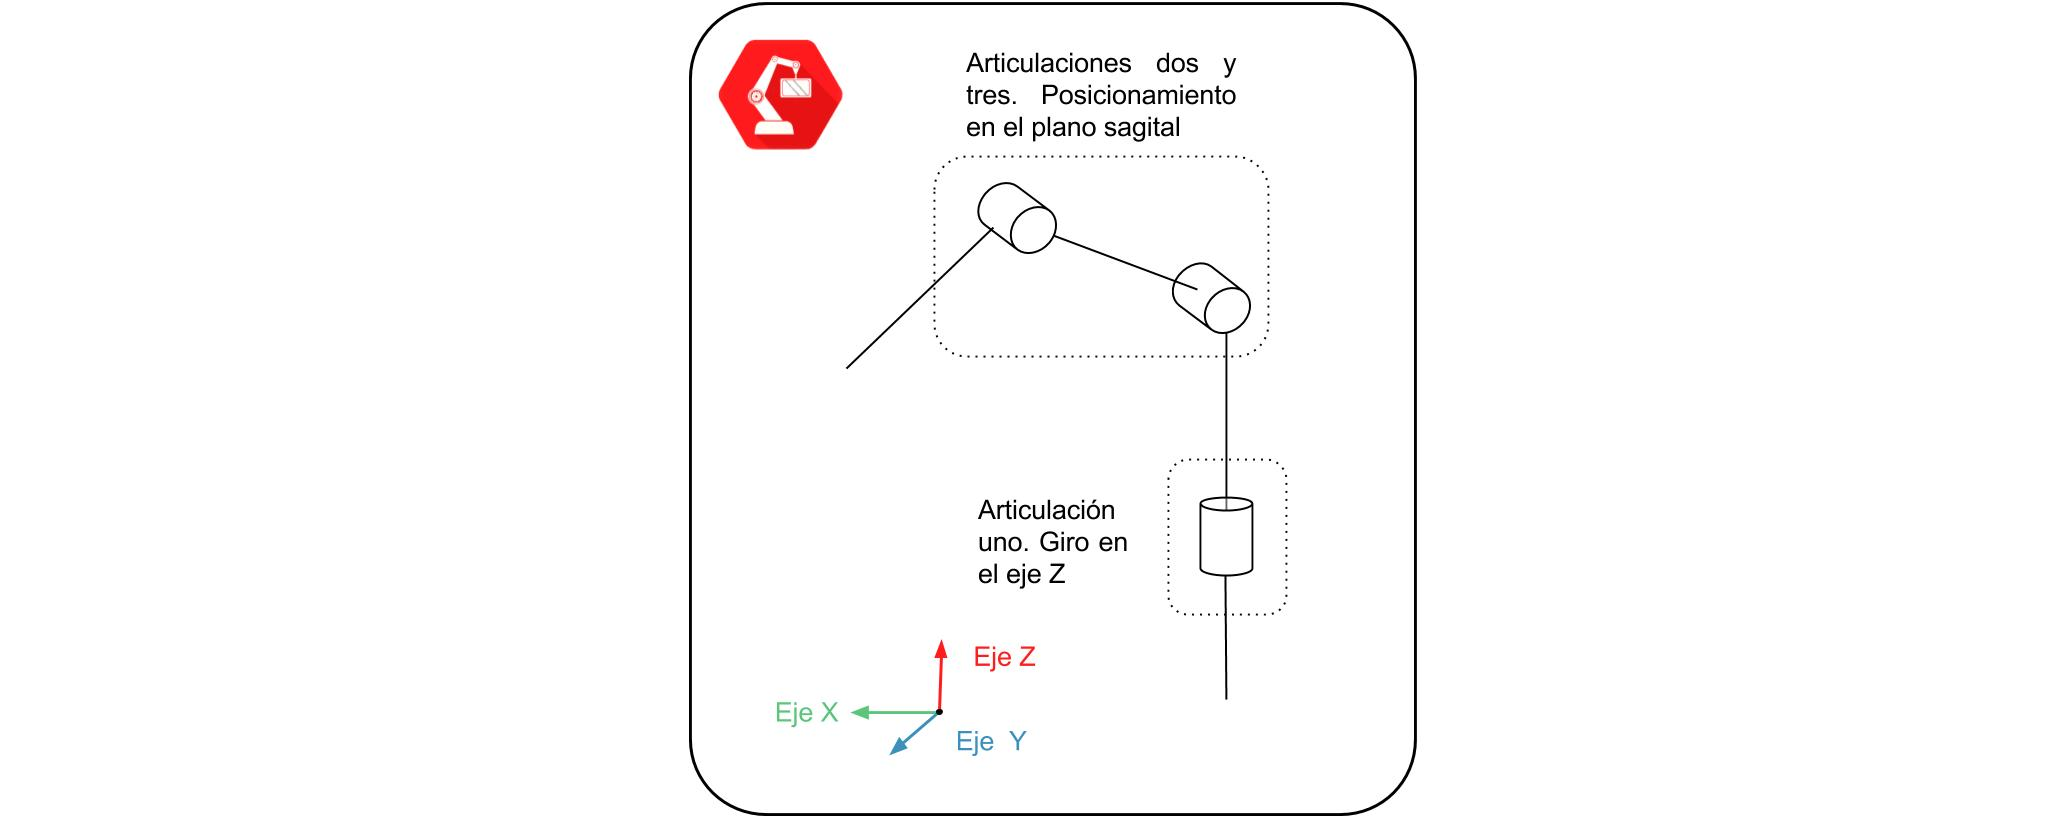
\includegraphics[width=\textwidth]{figuras/Imagenes_Mecanica/modelo_esquematico.jpg}
        \caption{Modelo de los grados de libertad de posición. Convencionalismos tomados}
        \label{fig:Mecanica:convenciones_generales}
        \immagesource{Autor}
    \end{figure}

    Como se ha comentado en secciones anteriores el brazo debe ser capaz de orientar la tablet de forma que ésta sea capaz de \textit{ver} y seguir los ojos del paciente. Aunque el brazo podría anclarse a diferentes estructuras de ahora en adelante se centra la justificación y desarrollo en el caso de uso sobre una camilla. Este caso es el que requiere mayor longitud de trabajo de forma que las dimensiones del brazo deberám permitirle abarcar de un lado a otro de la camilla.
    \\

    Este espacio de trabajo definido, que deberá abarcar aproximadamente $90cm$ (la mayoría de camas y camillas tienen esta medida), implica unas dimensiones de los eslabones del brazo considerables. Como se ha visto en capítulos anteriores el peso del prototipo es un factor importante tanto para la seguridad del usuario como para que pueda ser desplazado por unos motores de bajo par.
    \\

    La transimisión mecánica del movimiento debe optimizarse para ser capaz de mover el brazo; este trabajo se verá simplificado a su vez aligerando, cuando sea posible, la estructura del mismo. Como material estructural base se han elegido perfiles de aluminio de sección cuadrada (se describen en detalle en el capítulo \completar junto con el resto de materiales). Estos perfiles presentan una alta resistencia y capacidad de carga a la vez que un peso reducido.
    \\

    El material estructural definido se complementa con otra serie de piezas diseñadas específicamente para este proyecto (se puede ver el anexo \ref{app:listadoPiezas} para ver estas piezas). En este caso, por su versatilidad se utilizarán piezas modeladas digitalmente e Impresas en 3D posteriormente. De igual manera parte del diseño se apoya en piezas de metacrilato cortado con láser.
    \\

    Aunque el peso del brazo completo se estima será reducido, la transmisión mediante cuerdas debe ser completamente fiable. Debido a las dimensiones con las que se trabaja se ve inviable el uso de cadenas o cuerdas de gran grosor; es por eso que se ha optado por utilizar hilo de \ingles{kevlar} de un milímetro de grosor.
    \\

    Aunque supone anticipar parte del desarrollo que se verá a continuación, a modo de lista se pueden resumir los materiales necesarios a nivel constructivo del proyecto en:
    \begin{itemize}
        \item Barras de aluminio de sección cuadrada de 1/2"x1m (lado de la sección x longitud).
        \item Rodamientos de bolas de 4mm x 13mm (diámetro interior X diámetro exterior)
        \item Rodamientos de bolas de 3mm x 10mm (diámetro interior X diámetro exterior)
        \item Rodamiento axial de 37.5mm x 52mm (diámetro interior X diámetro exterior)
        \item Barras de acero macizo cilíndricas de 4mm de diámetro
        \item Barras de acero macizo cilíndricas de 3mm de diámetro
        \item Piezas impresas en impresora 3D. (Lista detallada en el Anexo \ref{app:listadoPiezas})
        \item Piezas de metacrilato cortadas con láser. (Lista detallada en el Anexo \ref{app:listadoPiezas})
        \item Tornillería: tornillos y tuercas de diferentes métricas.
        \item Hilo de kevlar.
        \item Poleas de acetal de 4.9mm x 21.8mm (diámetro interior X diámetro exterior).
        \item Soporte de sombrilla. La base sobre la que se apoye el brazo debe ser capaz de soportarlo en una posición de trabajo en todo momento. Para no fijar ni imponer ningún tipo de anclaje (a superficie plana, anclaje a una camilla, etc) se ha optado por esta solución para el desarrollo del prototipo.
    \end{itemize}

    En el capítulo \ref{chap:Gestion}, concretamente en la tabla \ref{tab:presupuesto}, están reflejados los detalles técnicos de estos materiales así como las referencias de compra, cantidades necesarias y precios.
 
\section{Filosofía y justificación de diseño} \label{sec:Mecanica:filosofia_diseno}

    Tal y como se ha adelantado en el capítulo introductorio el software empleado para modelar el brazo robótico es Autodesk Inventor. Este programa es especialmente potente para modelado paramétrico; esto significa que permite definir una serie de parámetros que serán utilizados para definir las medidas de los bocetos. Un diseño bien modelado parametricamente permite mucha flexibilidad a la hora de modificar ciertas medidas como pueden ser agujeros para tornillería, ejes u holguras.
    \\

    El modelado de todas las piezas ha seguido esta filosofía de parametrización y dependencia entre las piezas de forma que el diseño sea lo más flexible posible en cuanto a modificación de medidas. En la figura \ref{fig:Mecanica:diseno_parametrico} se puede ver a modo de ejemplo parte de la lista de parámetros definida.

    \begin{figure}[H]
        \centering
        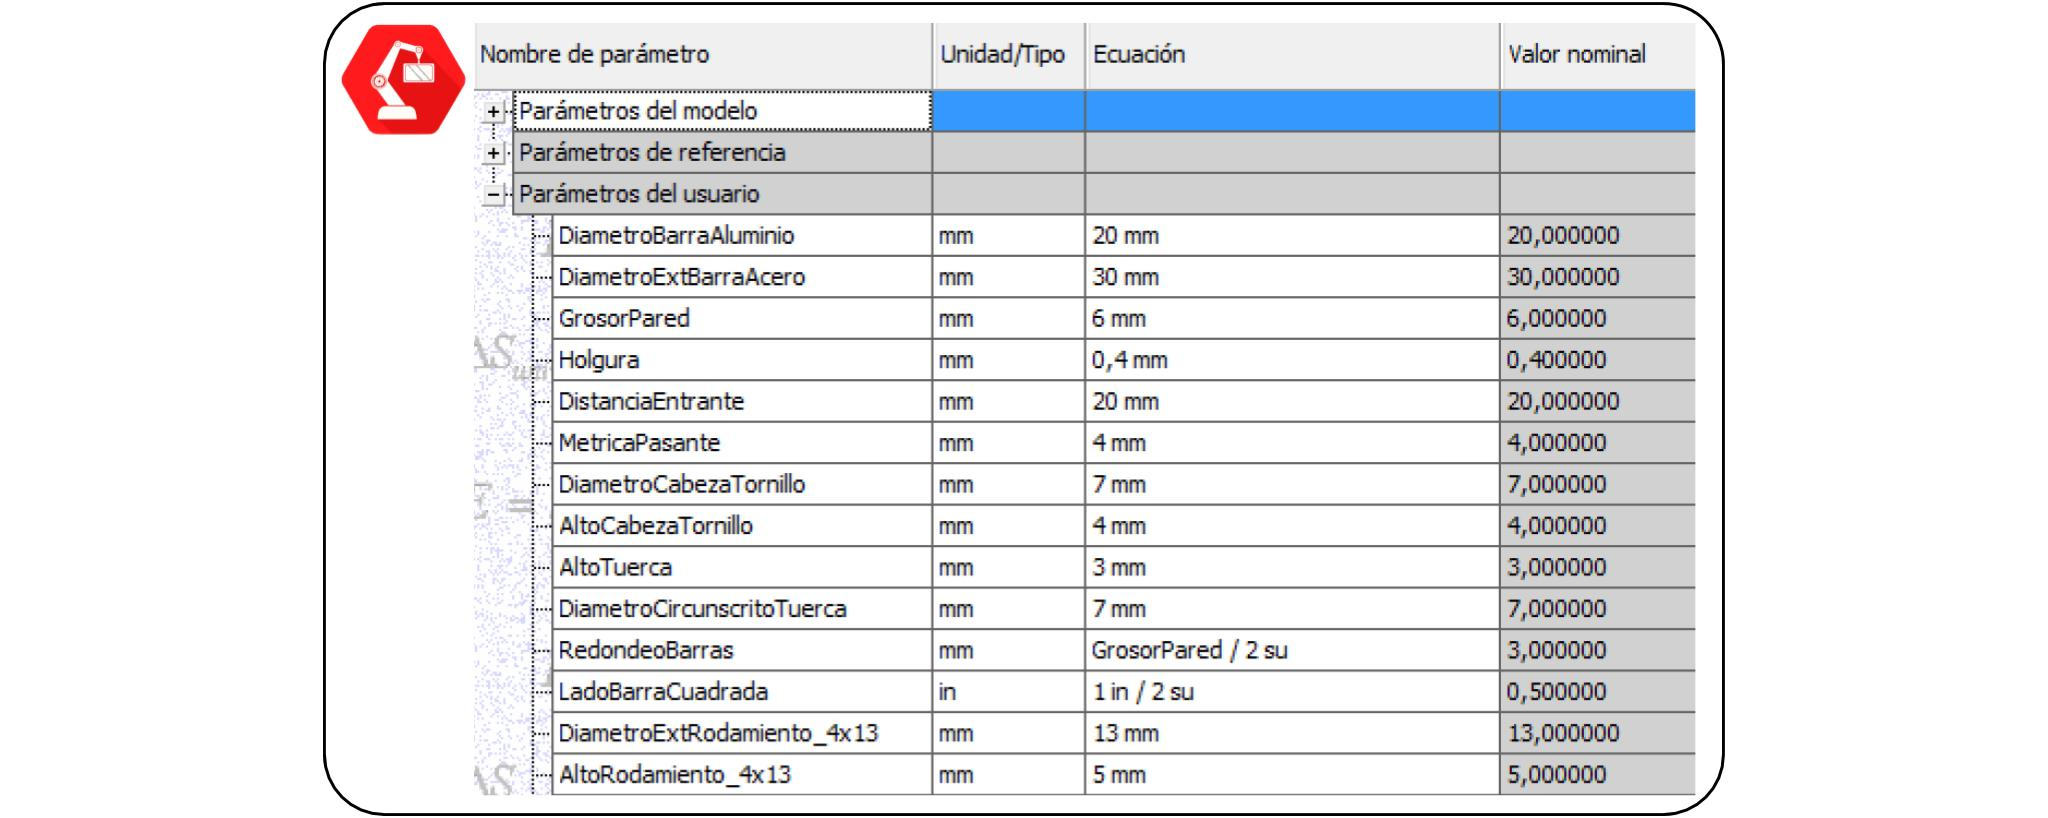
\includegraphics[width=\textwidth]{figuras/Imagenes_Mecanica/diseno_parametrico.jpg}
        \caption{Ejemplo de parámetros definidos en Inventor}
        \label{fig:Mecanica:diseno_parametrico}
        \immagesource{Autor}
    \end{figure}

\subsection{Realidad de las formas}
    Cualquier diseño de producto, incluso desde una más puramente perspectiva técnica incluye a su vez consideraciones sobre el diseño estético del mismo. Para este proyecto se ha intentado respetar la verdad de las formas predominantes tanto a nivel estructural como en el entorno de trabajo.
    \\

    Como ya se ha visto, la base estructural del prototipo está conformada por barras de aluminio de sección cuadrada. Unido a la predominancia de formas rectangulares y/o cuadradas en una habitación de hospital (figura \ref{fig:Mecanica:verdad_formas}) se ha optado por un diseño basado en prismas rectangulares, con un aspecto más \ingles{retro}.
    \\

    A nivel bibliográfico y del estado del arte estudiado se puede observar una tendencia a formas más suavizadas en muchos de los casos. En este proyecto se busca un contraste entre las formas que caracterizan al ser humano, más suavizadas y con geometrías complejas, en contraposición con las formas que definen el prototipo, formas geométricas y angulares.

    \begin{figure}[H]
        \centering
        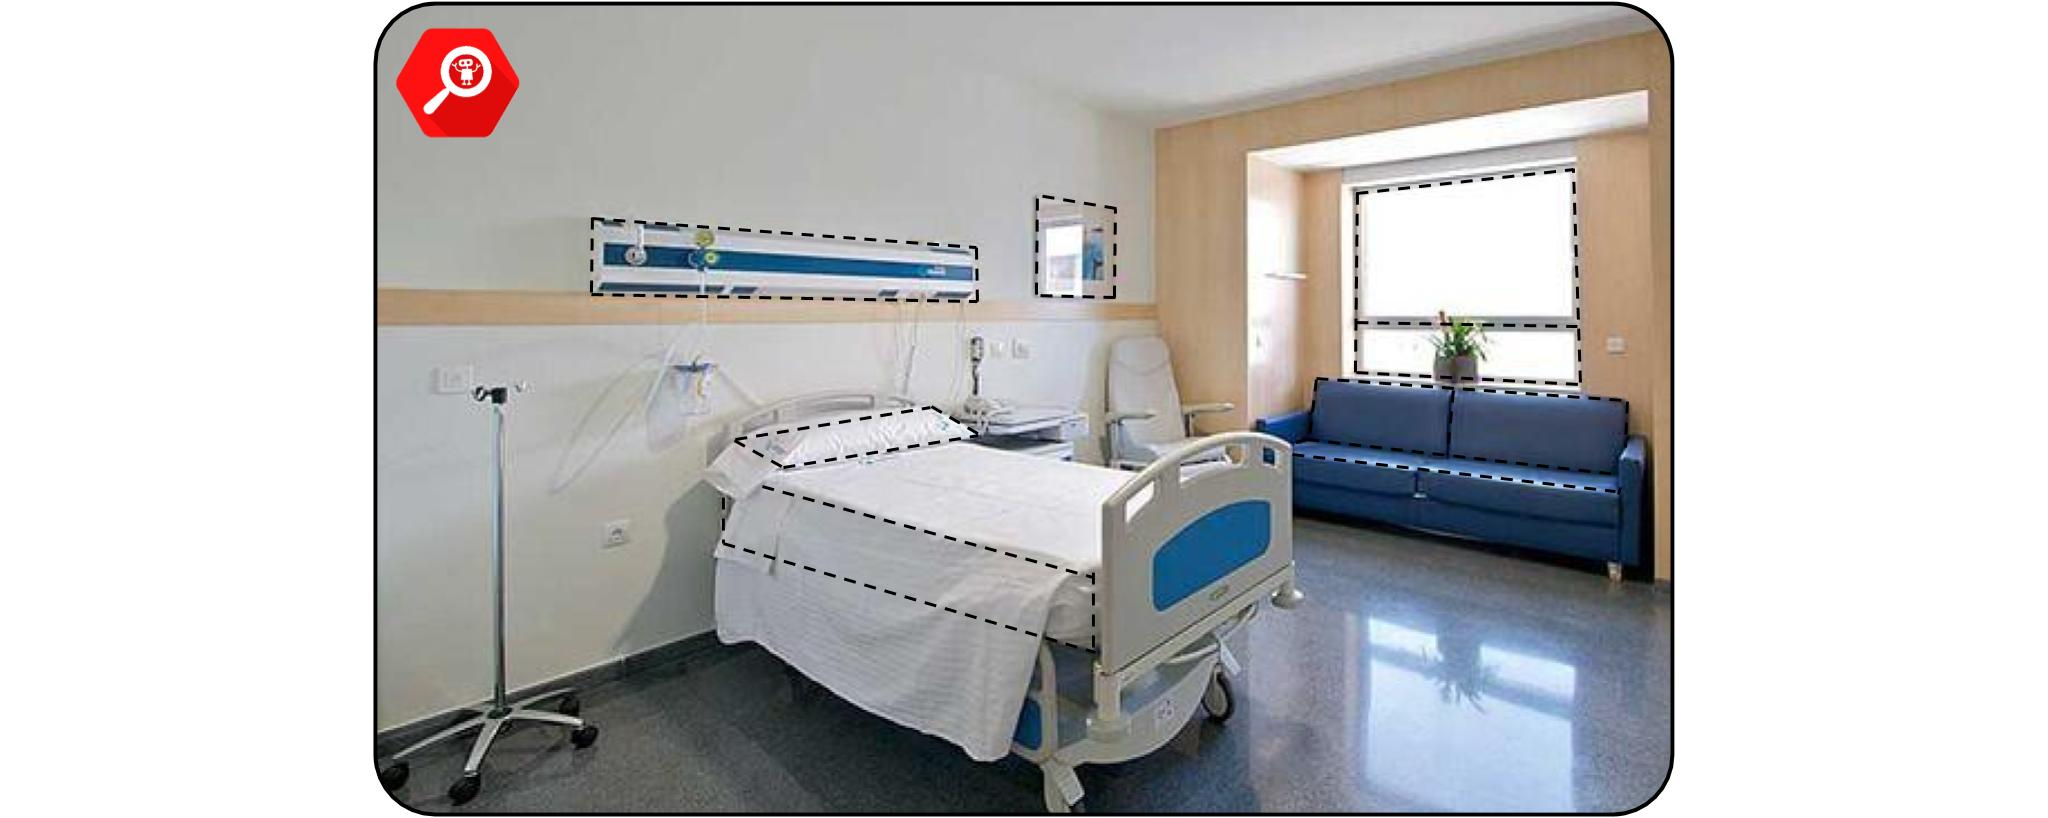
\includegraphics[width=\textwidth]{figuras/Imagenes_Mecanica/verdad_de_formas.jpg}
        \caption{Predominzancia de formas rectangulares en el entorno de trabajo}
        \label{fig:Mecanica:verdad_formas}
        \immagesource{Imagen de consalud.es, editada posteriormente por el Autor}
    \end{figure}

\section{Articulación uno. Giro en el eje Z} \label{sec:Mecanica:articulacion_uno}
    Junto con las articulaciones dos y tres, descritas en la Sección \ref{sec:Mecanica:articulacion_dostres} están consideradas como los grados de libertad que gestionan la posición del extremo del robot en un espacio tridimensional. En adelante se las podrá denominar también "grados de libertad de posición".
    \\

    Esta articulación está actuada por un \ingles{Servo G15 Cube} (descrito en la Sección \ref{sec:Introduccion:materiales_software}. El movimiento de dicho servo se transmite a la articulación a través de un juego de ruedas que, solidarias a la parte superior (parte móvil) de la articulación y por rozamiento, transmiten el movimiento hasta la pista inferior (parte fija a la base del robot).
    \\

    De esta forma aseguramos que el usuario, en cualquier momento, podrá desplazar el robot superando el rozamiento de esta cadena de transmisión anulando, en caso de estar en proceso, el movimiento que pueda estar efectuando el \glosario{servo}.
	\\
	En la figura \ref{fig:Mecanica:giro_z} se puede ver en detalle el montaje de dicha estructura. Las piezas de la imagen se encuentran, con la misma referencia, en el Anexo \ref{app:listadoPiezas}.

	\begin{figure}[H]
		\centering
		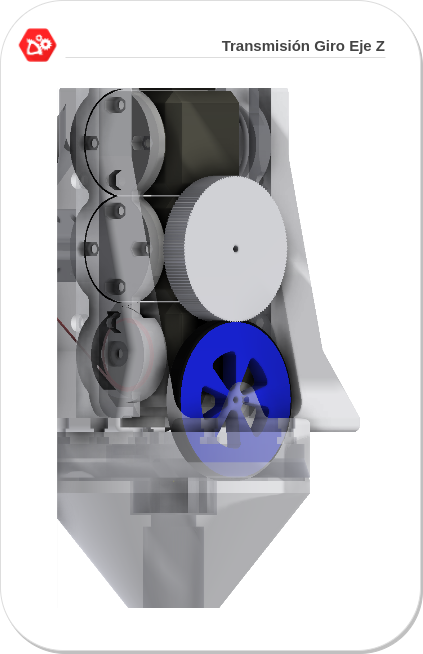
\includegraphics[width=0.5\textwidth]{figuras/Imagenes_Mecanica/RuedasGiroZ.png}
		\caption{Montaje de la transmisión del movimiento del servo a la articulación encargada de girar en Z}
		\label{fig:Mecanica:giro_z}
		\immagesource{Autor}
	\end{figure}

	El apoyo del peso en la última versión se hace sobre un rodamiento \completarCon{coaxial? o como se llamaba?} para conseguir un apoyo completo. Previamente se contempló la posibilidad de utilizar ruedas sobre un carril, de forma que se mantenía una estructura similar a la rueda motriz. En este caso tras probar ambas opciones se optó por colocar la rueda motriz en el lado sobre el que cae la carga del brazo al extenderse para maximizar el apoyo. Este aspecto se ha mantenido al integrar el rodamiento, que asegura un mayor apoyo que las ruedas aun reduciendo el diámetro de dicho apoyo (dificultando la distribución de cargas).

	\completarCon{Imagen de las ruedas con las distintas configuraciones de carga y rueda motriz}

	\completarCon{Imagen de como afecta el cambio de diámetro del apoyo}

\section{Articulaciones dos y tres. Posicionamiento en el plano sagital} \label{sec:Mecanica:articulacion_dostres}
    Estas dos articulaciones son las encargadas de posicionar el extremo en el plano sagital del robot.
    \\

    \begin{figure}[H]
       	\centering
       	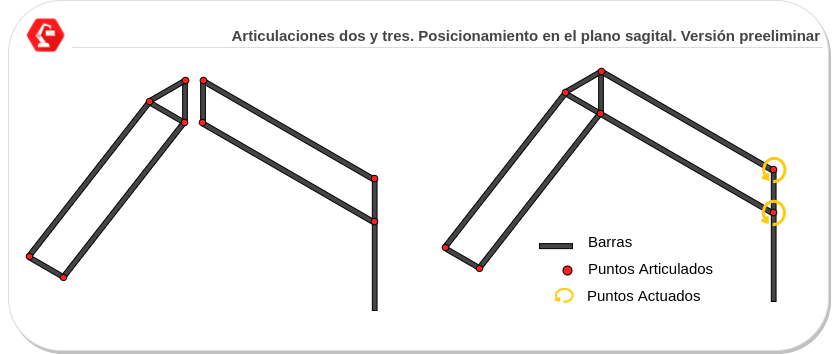
\includegraphics[width=0.9\textwidth]{figuras/Imagenes_Mecanica/mecanismos_4_barras_triangulo.png}
       	\caption{Esquema de la cadena cinemática correspondiente a los \completarCon{Glosario a GDL} dos y tres. Idea preliminar}
       	\label{fig:Mecanica:4_bar_mecanism_triangle}
       	\immagesource{Autor}
    \end{figure}

    Están formadas por dos mecanismos de cuatro barras acoplados en serie. Tienen la particularidad de que las barras son iguales dos a dos, de forma que las barras se mantienen siempre en paralelo.
    \\

    \begin{figure}[H]
    	\centering
    	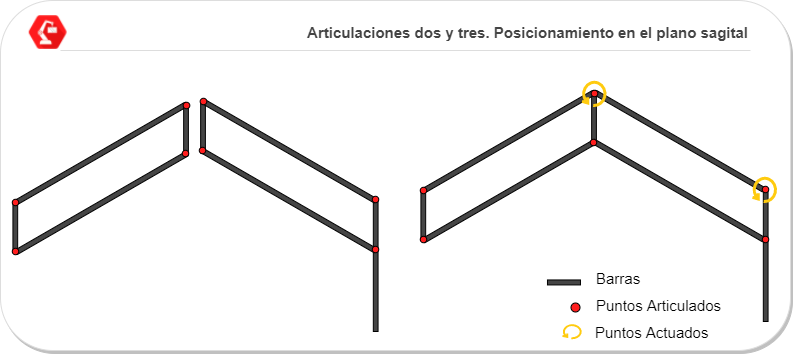
\includegraphics[width=0.9\textwidth]{figuras/Imagenes_Mecanica/mecanismos_4_barras.png}
    	\caption{Esquema de la cadena cinemática correspondiente a los \completarCon{Glosario a GDL} dos y tres}
    	\label{fig:Mecanica:4_bar_mecanism}
    	\immagesource{Autor}
    \end{figure}

    Como se puede ver en la figura \ref{fig:Mecanica:4_bar_mecanism} y \ref{fig:Mecanica:4_bar_mecanism_triangle} la actuación se realiza sobre cada articulación en los puntos marcados. El movimiento se transmite desde los servos ubicados en la base de la articulación 1 hasta las mismas a través de un hilo de \ingles{kevlar}. Un sistema de poleas amplifica y redirige el par hasta los mismos. En la figura \ref{fig:Mecanica:transmision_poleas_cuerda} se puede ver como se redirecciona el hilo desde la base en dirección hacia las articulaciones superiores.

   	\begin{figure}[H]
   		\centering
   		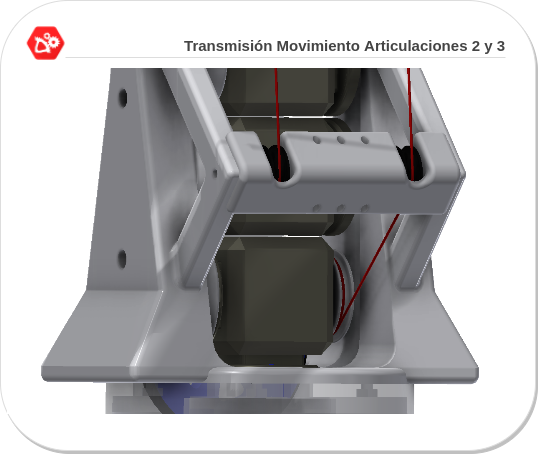
\includegraphics[width=0.6\textwidth]{figuras/Imagenes_Mecanica/TransmisionMotorArticulacion.png}
   		\caption{Montaje de la transmisión del movimiento de los servos a las articulaciones 2 y tres.}
   		\label{fig:Mecanica:transmision_poleas_cuerda}
   		\immagesource{Autor}
   	\end{figure}

   	En las figuras \ref{fig:Mecanica:4_bar_mecanism} y \ref{fig:Mecanica:4_bar_mecanism_triangle} se muestran dos posibles configuraciones mecánicas que se han probado. En la primera, ubicada al principio de la sección (figura \ref{fig:Mecanica:4_bar_mecanism_triangle}) se cuenta con la ventaja de actuar ambas articulaciones sobre el mismo punto de actuación, facilitando la realimentación así como el paso de cables (tanto eléctricos como de transmisión mecánica). Como se puede ver la orientación del extremo depende de los ángulos del triángulo ubicado en el equivalente a la tercera articulación, donde se redirecciona el giro. En este caso las barras a partir de dicho triángulo se encuentran soldadas para hacer la actuación sobre el punto ya mencionado. Otra configuración posible, mostrada en la figura \ref{fig:Mecanica:4_bar_mecanism}, aprovecha esta propiedad de mantener la orientación del extremo a lo largo de la cadena cinemática haciendo que, desde el inicio todas estas conexiones se hagan de forma perpendicular al plano del suelo. De esta forma se puede asegurar que el extremo de dicha cadena mecánica siempre se mantendrá perpendicular al suelo consiguiendo un desacople absoluto de los grados de posición del robot de los grados de libertado que controlan la orientación. En este caso, las barras del extremo no se encuentran soldadas como en el primer caso por lo que el control de la tercera articulación no se puede hacer sobre el mismo punto, como se hacía antes si no que se lleva a la unión de ambos mecanismos. Se ha dado finalmente más peso a la característica de mantener la orientación por facilitar mucho el desarrollo matemático y de control futuros.

\section{Posicionamiento de sensores y actuadores} \label{sec:Mecanica:sensores_actuadore}

	Como e ha anticipado en secciones anteriores los tres motores correspondientes al giro en el eje Z así como el posicionamiento en el plano sagital están ubicados sobre la primera articulación uno encima de otro formando una torre. Desde ahí se dirige a través de hilos el par motor del primer y tercer servo hasta las articulaciones que dos y tres y a través de fricción por ruedas hasta el giro en el eje Z. En la figura \completar se puede ver en detalle dicho montaje así como la fijación a la base de giro.
	\\

	\completarCon{Imagen en detalle de la torre de motores}

	Las articulaciones realimentadas son la articulación dos y la articulación tres, que llevan una realimentación de posición articular a través de un potenciómetro en cada una. El primer grado de libertad, el encargado del giro en el eje Z no está realimentado externamente. En este caso se cuenta con la información proporcionada por el servo y finalmente, la proporcionada por la tablet en el extremo.
	\\

	En el caso de la segunda articulación el potenciómetro se conecta con la propia articulación a través de un juego de engranajes con una relación de \completar que maximiza el uso del potenciómetro, ajustando el rango de movimiento del mismo (\completarCon{cuantos grados gira?}) con el ángulo de giro de la articulación (\completarCon{cuantos grados gira?}). En el caso de la tercera articulación el eje del potenciómetro se encuentra en la misma línea que el eje de giro que se pretende realimentar, el giro es solidario a dicha barra por lo que la relación de giro es unitaria. En la figura \completar se pueden ver ambos montajes: a la derecha la articulación dos con el juego de engranajes; a la izquierda la articulación tres con la transmisión solidaria.

	\completarCon{Añadir fotos de como se enganchan ambos potenciómetros}

\section{Estudio de la cadena cinemática completa} \label{sec:Mecanica:cadena_cinematica}

\completarCon{Hablar de como se reduce la carga hasta los servos: columpios, poleas dobles, palancas, etc}
